{\documentclass[authoryear]{elsarticle}

\pagenumbering{gobble}


\makeatletter
\def\ps@pprintTitle{%
\let\@oddhead\@empty
\let\@evenhead\@empty
\def\@oddfoot{}%
\let\@evenfoot\@oddfoot}
\makeatother


\setlength\arraycolsep{2pt}
\setlength{\parskip}{1ex plus 0.5ex minus 0.2ex}
\usepackage{graphicx}
\usepackage{amsfonts}
\usepackage{multirow}
\usepackage{comment}

%\usepackage{chicago}
\bibliographystyle{chicago}



\newcommand{\eps}{\epsilon}
\newcommand{\cov}{{\rm cov}}
\newcommand{\nid}{{\rm NID}}
\newcommand{\diag}{{\rm diag}}
\newcommand{\E}{{\mathrm E}}
\newcommand{\R}{{\mathrm R}}
\newcommand{\RD}{{\tilde{\mathrm R}}}
\newcommand{\Q}{{\mathrm Q}}
\newcommand{\U}{{\mathrm U}}
\newcommand{\Ex}{{\cal E}}
\newcommand{\cor}{\mathrm{cor}}
\newcommand{\tr}{\mathrm{tr}}
\newcommand{\e}{\mathrm{e}}
\newcommand{\de}{\mathrm{d}}
\newcommand{\p}{\mathrm{P}}
\newcommand{\Ln}{\mathrm{Ln}}
\newcommand{\ra}{\varrho}

\newcommand{\minn}{\mathrm{min}_n}
\newcommand{\maxn}{\mathrm{max}_n}
\newcommand{\cq}{\ ,\qquad}
\renewcommand{\top}{T}
\newcommand{\var}{\mathrm{VaR}}

\newcommand{\bi}{\begin{itemize}}
\renewcommand{\i}{\item}
\newcommand{\ei}{\end{itemize}}


\newcommand{\ppo}[1]{|{#1}|^+}

\newcommand{\ssection}[1]{%
  \section[#1]{\textbf{\uppercase{#1}}}}
\newcommand{\ssubsection}[1]{%
  \subsection[#1]{\normalfont\textbf{#1}}}


%\renewcommand{\labelenumi}{(\roman{enumi})}

\newcommand{\eref}[1]{(\ref{#1})}
\newcommand{\fref}[1]{Figure \ref{#1}}
\newcommand{\sref}[1]{\S\ref{#1}}
\newcommand{\tref}[1]{Table \ref{#1}}
\newcommand{\aref}[1]{\ref{#1}}


\begin{document}


\begin{frontmatter}

\title{The tradeoff insurance premium as a two--sided generalisation of the distortion premium}


\begin{abstract}
This paper introduces and analyzes the ``tradeoff premium," generalising the loss aversion reserve, distortion premium, spectral risk, and their duals. The tradeoff premium is a weighted average loss where weights increase as loss outcomes deviate from a subjective ``loss appetite," rather than from zero. The U--shaped weights replicate subjective probability adjustment in cumulative prospect theory, and minimise pricing error in a competitive market where overpricing and underpricing are both undesired.
\end{abstract}

\begin{keyword}
Weighted premium; loss aversion reserve; distortion premium; spectral risk; two--sided; loss appetite.
\end{keyword}



\end{frontmatter}


\section{Introduction and overview}



Premium principles, or risk measures, map a loss distribution to a real number. The mapping is used to calculate insurance premiums or manage risk. An example premium principle is the loss aversion reserve \citep{choo2009loss}, a weighted average loss where weights are a non-decreasing function of the loss percentile rank. Loss aversion reserves are equivalent to distortion premiums \citep{wang1996pct} and spectral risks \citep{acerbi2002spectral}. Generalised premium principles based on weighted average losses are discussed in \citet{furman2008weighted}. \citet{gerber1985additive} discusses an alternative premium based on the certainty equivalent loss under utility theory, the exponential premium \citep{deprez1985convex} being a specific example. Other common premiums or risks are discussed in \citet{mcneil2005qrm} and \citet{young2004premium}, including Value--at--Risk, conditional--tail--expectation and the standard deviation premium. \citet{artzner1999cmr} discusses ``coherence" properties of a premium principle or risk measure, namely translation invariance, positive homogeneity, monotonicity, and subadditivity.

Existing premium principles and risk measures are mostly ``one--sided", focussing on large loss outcomes and adding a positive loading to the expected loss. In pricing, a positive loading avoids inevitable ruin in the long run. In risk management, a positive loading captures worse than expected losses, which are the main concern. For example, the loss aversion reserve (or distortion premium and spectral risk) magnifies higher loss percentiles. The standard deviation premium sets the loading as a positive multiple of standard deviation. Assuming a concave utility function, representing risk aversion, the certainty equivalent premium exceeds the expected loss. The Dutch premium \citep{van1992dutch} also assumes a positive loading above the expected loss, based on a multiple of the expected excess loss.

A ``two--sided" premium reflecting the importance of smaller loss outcomes, and potentially having a negative loading, is required for business reasons. In a competitive market, a negative loading may apply in the short term to increase business volume or to avoid loss of business, the latter if other market players are also applying negative loadings. Hence conflicting considerations exist -- a positive loading is financially sustainable in the long term, however competitive pressure may force a negative loading to ensure short term survival. A negative loading may sustain for a longer term if the financial loss is offset by profit from other products with positive loading.

The tradeoff premium (ToP) is a novel premium principle addressing ``two--sided" concerns highlighted in the previous paragraph. The ToP is a weighted average loss, with U--shaped weights increasing as loss outcomes deviate from a subjective ``loss appetite." U--shaped weights reflect the importance of both small and large loss outcomes, and are consistent with cumulative prospect theory \citep{tversky1992apt} where extreme outcomes (both positive and negative) are magnified and moderate outcomes are diminished.

The ToP is shown to reduce with loss appetite, with zero loss appetite yielding the loss aversion reserve (equivalently distortion premium or spectral risk). A maximum loss appetite implies monotonic decreasing weights, and yields a negative loading. In addition the resulting ToP is shown to be the dual \citep{wang2000cdo} of the distortion premium with zero loss appetite.

Examples in this paper express the ToP as a two--sided generalisation of one--sided premiums or risks, including Value--at--Risk, conditional--tail--expectation and expected--maximal--loss \citep{choo2009loss}. The two--sided generalisation reflects the undesirability of both small and large loss outcomes, with the loss appetite controlling their relative representation in the ToP.

The equilibrium ToP corresponds to the loss appetite. Hence at equilibrium, the appetite for loss is equal to the premium collected. Undesired deviations of loss outcomes from the loss appetite represent premium surplus or shortfall. The equilibrium ToP is shown to be a tail--magnified measure of central tendency, refining the mean and median measures. Hence for a right skewed loss distribution, the equilibrium ToP exceeds the expected loss, and vice versa for a left skewed loss distribution.

The remaining paper is structured as follows. Section \aref{s_definition} defines, illustrates and justifies the ToP. Section \aref{s_properties} discusses properties of the ToP, in particular coherence. The ToP does not satisfy the subadditivity property of coherence, due to its two--sided nature. Section \aref{s_equilibrium} discusses the equilibrium ToP. Section \aref{s_otherlinks} identifies links between the ToP and existing literature. Section \aref{s_decompose} decomposes the ToP into the expected loss, and a discount and loading respectively reflecting loss volatility below and above the loss appetite. Section \aref{s_numericaleg} provides a numerical example of the ToP using a gamma loss distribution and power aversion pattern. Section \aref{s_conclusion} concludes.



\section{The tradeoff premium}\label{s_definition}


The tradeoff premium (ToP) is a weighted premium \citep{furman2008weighted}.   ToP  generalises loss aversion reserves \citep{choo2009loss}, distortion premiums \citep{wang1996pct} and spectral risks \citep{acerbi2002spectral} by assigning higher penalty weights to loss outcomes further from a ``loss appetite" rather than to larger loss outcomes. Penalty weights forming the ToP are aligned with cumulative prospect theory \citep{tversky1992apt}, where extreme outcomes, relative to a reference point, are magnified and moderate outcomes are diminished. The ToP also minimises pricing error in a competitive market.

To explain the ToP, first consider the loss aversion reserve of a random loss  $x\geq 0$ with distribution function $F$ and percentile rank $u\equiv F(x)$.  Then $u$ is uniformly distributed on the unit interval and indicates ``loss severity," with $0$ being least severe and $1$ being most severe. Given an increasing aversion function $\phi\geq0$ integrating to one, the loss aversion reserve of $x$ is
\begin{equation}\label{dp}
\E\{x\phi(u)\}= \int_0^\infty\left[ 1-\Phi\{F(x)\} \right]\de x =\int_0^1 V_u\phi(u) \de u  \;,
\end{equation}
$$
\Phi(u)\equiv \int_0^u \phi(v) \de v\cq  V_u\equiv F^-(u)\ ,
$$
where $\E$ computes expectation and $V_u$ is the Value--at--Risk or VaR \citep{mcneil2005qrm} with sufficiency probability $u$.  The second and third expressions in \eref{dp} are  the distortion premium and spectral risk of $x$, respectively.

The loss aversion reserve \eref{dp} is a weighted average loss with higher weight on larger severities. Weights are on average one: $\E\{\phi(u)\}=1$, since $\phi$ integrates to one. The distortion premium is the expected loss computed using a distorted distribution $\Phi\circ F$ dominating $F$, noting $\Phi$ is convex. The spectral risk is a weighted average of VaRs where higher VaRs are weighted more heavily. Hence loss aversion reserves, distortion premiums and spectral risks are ``one--sided", concerned only with larger severities. Concern is characterised  by $\phi$ reweighing initially  equally weighted VaRs or severities. Equal weighting $\phi=1$ leads to the original expected loss $\E(x)$. \cite{choo2009loss} shows the equivalence between loss aversion reserves, distortion premiums and spectral risks.

``Loss appetite" is central to the ToP. To introduce the concept of loss appetite, loss aversion reserves assume zero loss appetite.  Then larger losses are always feared more and penalised more heavily. However a positive loss appetite may be relevant or even optimal in a business setting. In a competitive market, premiums may be deliberately reduced to win or prevent loss of market share. Premium reduction is achieved with a positive loss appetite. Penalty weights decrease up to the loss appetite, and increase thereafter. Maximum loss appetite occurs if  penalty weights always decrease with severity and contrasts with zero loss appetite where penalty weights always increase with severity. The aversion function redistributes weights, in regions below and above loss appetite.

To achieve the above redistribution of penalty weights first define ``satiation error" based on loss severity $u$:
$$
\psi_\ell(u) \equiv (u\leq \ell)\frac{\ell-u}{\ell}+(u>\ell)\frac{u-\ell}{1-\ell}\cq 0\leq \ell\leq 1\ ,
$$
where the above bracketed inequalities are indicators. Here $\ell$ is a subjectively specified loss appetite on the percentile rank scale, with $\ell=0$ indicating no appetite for losses and $\ell=1$ indicating a complete appetite for losses.  The deviation $u-\ell$ is standardised so that $\psi_\ell(0)=\psi_\ell(1)=1$ with linear behaviour over the segments $[0,\ell]$ and $[\ell,1]$.

Similar to loss severity $u$,  satiation error $\psi_\ell(u)$ is uniformly distributed over the unit interval. Satiation error is also uniform over $u\le\ell$ and over $u>\ell$. Zero loss appetite, $\ell=0$,  reduces  satiation error to loss severity: $\psi_0(u)=u$.   Maximum loss appetite, $\ell=1$ yields satiation error $\psi_1(u)=1-u$.  The role and selection of the loss appetite parameter $\ell$ is further discussed below.

The ToP is defined analogous to \eref{dp} by imposing an aversion function $\phi$  on satiation error $\psi_\ell(u)$, yielding
\begin{equation}\label{tradeoff}
\top_\ell \equiv \E\{x\phi_\ell(u)\} = \int_0^\infty \left[1-\Phi_\ell\{F(x)\}\right] \de x = \int_0^1 V_u\phi_\ell(u) \de u
%=\int_0^1\left\{1-\Phi_\ell(u)\right\}V_u'
\;,
\end{equation}
where
$$
\phi_\ell\equiv \phi\circ \psi_\ell \cq \Phi_\ell(u) \equiv \int_0^u \phi_\ell(v) \de v \;.
$$
Note $\top_0$ reduces to the expression in \eref{dp} since $\phi_0(u)=\phi(u)$. Conversely maximum loss appetite $\ell=1$ yields satiation error $\phi_1(u)=\phi(1-u)$. The resulting ToP,  $\top_1$, is the ``dual'' of the original distortion premium \citep{wang2000cdo}:
$$
\int_0^\infty \left[1-\Phi^*\{F(x)\}\right] \de x  \cq \Phi^*(u)\equiv 1-\Phi(1-u) \;.
$$

The ToP is a ``two--sided" generalisation of the loss aversion reserve, noting weights $\phi_\ell(u)=\phi\{\psi_\ell(u)\}$ increase as loss severity $u$ deviates from loss appetite $\ell$, rather than from zero. Overall weights below and above the loss appetite are
$$
\int_0^\ell \phi_\ell(u) \de u = \ell \cq \int_\ell^1 \phi_\ell(u) \de u = 1-\ell \;,
$$
respectively, noting satiation error $\psi_\ell(u)$ is uniform over both $u\leq\ell$ and $u>\ell$. Hence piecewise uniformity of $\psi_\ell(u)$ preserves the overall weight placed on severities below and above the loss appetite $\ell$. The loss appetite $\ell$ serves to  redistribute severity weights, using the aversion function $\phi$.  An example illustrating the ToP is shown in the following subsection. Subsequent subsections further justify the formulation of the ToP based on cumulative prospect theory and minimisation of pricing error in a competitive market.


\subsection{Minmax ToP example}


The following example illustrates $T_\ell$ given power aversion function $\phi(u)=nu^{n-1}$ with $n\ge 1$.  In this case
$$
\top_\ell=\ell\E\left\{\left.\min_{i=1,\ldots,n}(x_i)\right|x_i\leq V_\ell\right\}
+(1-\ell)\E\left\{\left.\max_{i=1,\ldots,n}(x_i)\right|x_i>V_\ell\right\} \;,
$$
where  the $x_i$ are $n$ independent copies of $x$.  With minimum and maximum loss appetite, or $\ell=0,1$, the ToPs are respectively
$$
\top_0=\E\left\{\max_{i=1,\ldots,n}(x_i)\right\} \cq \top_1=\E\left\{\min_{i=1,\ldots,n}(x_i)\right\} \;.
$$
Further  for $0\leq \ell\leq 1$, $\top_1\leq \top_\ell \leq \top_0$.   If $n=1$ then $\phi(u)=1$  and the ToP is, for all $\ell$,
$$
\top_\ell=\ell\E(x|x\leq V_\ell)+(1-\ell)\E(x|x>V_\ell) = \E(x) \;.
$$
The following key properties of the ToP are inferred from the above example, and are formalised in subsequent sections:
\bi
\i The ToP is formed by combining ``aversion adjusted" conditional expected losses below and above the loss appetite. The expected loss below the loss appetite is reduced by assuming the expected minimum. The expected loss above the loss appetite is raised by assuming the expected maximum. Without aversion adjustment $(n=1)$ the ToP is the expected loss.

\i Loss appetite $0\leq \ell\leq 1$ controls the size of the ToP. $\top_\ell$ is at maximum if  $\ell=0$, that is if there is no appetite for loss.  Increasing loss appetite reduces the ToP. A proof is shown in \sref{s_properties}.

\i Relative left and right tail skewness about $\ell$ also affect the ToP, given the loss appetite.  Increasing the skewness of the right tail while keeping $\E(x)$ constant increases the expected maximum of losses above loss appetite, resulting in a higher ToP.

\i Increasing loss aversion by increasing $n$ in $\phi(u)=nu^{n-1}$ accentuates the impact of relative tail skewness on the ToP. Consider a right skewed loss distribution about $\ell$. Increasing $n$ has a greater impact on the expected maximum of losses above the loss appetite than the expected minimum of losses below the loss appetite, thus increasing the ToP overall. With neutrality $n=1$ or $\phi=1$, relative tail skewness is ignored and the ToP is always the expected loss $\E(x)$.

\i The same aversion attitude applies to losses below and above the loss appetite. In this example aversion adjustment focusses on the expected maximum or minimum over $n$ copies.



\ei



\subsection{ToP and cumulative prospect theory}

In cumulative prospect theory, extreme outcomes are over--weighted while average outcomes are under--weighted. This psychological phenomenon is represented by a U--shaped weight function on probabilities, and a S--shaped transformation of cumulative probabilities. The ToP effects a similar modification. The weight function $\phi_\ell$ in the first expression of the ToP in \eref{tradeoff} is U--shaped: decreasing below $\ell$ and increasing above $\ell$. In the second expression, the transformation $\Phi_\ell$ applied to the distribution $F$ is S--shaped: concave below $\ell$ and convex above $\ell$. Left and right panels in \fref{aversiongraph} illustrate the U--shaped $\phi_\ell$ and S--shaped $\Phi_\ell$, respectively, assuming $\phi(v)=5v^4$, for various values of $\ell$.
\begin{figure}
  \begin{center}
    \begin{tabular}{cc}
      \resizebox{60mm}{!}{\includegraphics{aversionvarypi.eps}}
      \resizebox{60mm}{!}{\includegraphics{CPTvarypi.eps}} \\
    \end{tabular}
    \caption{Plots of $\phi_\ell(u)$ (left panel) and $\Phi_\ell(u)$ (right panel) against $u$ assuming $\phi(v)=5v^4$ and $\ell=0.25$, $0.5$ and $0.75$.}
    \label{aversiongraph}
  \end{center}
\end{figure}


\subsection{ToP and the minimisation of pricing error}

In a competitive market, overpricing leads to  loss of business. Hence smaller loss outcomes are feared. Larger loss outcomes are also feared, due to underpricing and financial loss. Loss appetite $\ell$ and the associated VaR $V_\ell$ sets the boundary between perceived ``small" and ``large" losses. A lower loss appetite $\ell$ yields a higher proportion of ``large" losses and vice versa. U--shaped penalty weights $\phi_\ell(u)$ models the undesirability of various severities.

Given premium $\pi$,  then
\begin{equation}\label{pe}
\E\left\{(\pi-V_u)^2\phi_\ell(u)\right\}= \int_0^1 (\pi-V_u)^2  \de \Phi_\ell(u) \;,
\end{equation}
is the overall pricing error. Squared pricing errors $(\pi-V_u)^2$ are weighed according to the aversion function $\phi_\ell$, given loss appetite $\ell$.  Large pricing errors, those associated with smaller or larger severities $u$, are featured more prominently in the overall pricing error via larger squared differences and penalty weights. The ToP, $\top_\ell$, is  that premium $\pi$ minimising overall pricing error in \eref{pe}.


\subsection{Role and selection of loss appetite}

The loss appetite parameter $\ell$ is central to the ToP and distinguishes it from one--sided premium principles.   As mentioned just after \eref{tradeoff}, zero loss appetite $\ell=0$ yields the usual distorted premium, whereas the dual is obtained with $\ell=1$, the maximum loss appetite.

Loss appetite $\ell$ is  subjectively selected  within the unit interval. The chosen $\ell$ is a neutrality, ``preference" or ``comfort" point  with no aversion: $\phi_\ell(\ell)=0$ and no distribution adjustment: $\Phi_\ell(\ell)=\ell$.  Aversion increases as  $|u-\ell|$ increases.

Loss appetite $\ell$  balances  the fear of ``small" severities,  suggesting   overpricing and  possible loss of business, relative to the fear of  ``large" severities, indicating underpricing and an overall loss.  A low loss appetite, $\ell\approx 0$,  indicates little fear of overpricing and loss of business, and large fear of underpricing and overall loss and vice versa. In the above example, the loss appetite is the weight attached to aversion adjusted expected losses below the loss appetite, while the complement is the weight attached to the corresponding expectation of losses above the loss appetite.

An equilibrium occurs if $F(\top_\ell)=\ell$, that is if $\top_\ell=V_\ell$, the VaR at $\ell$. In this case the loss appetite $\ell$ equals the probability of an adequate premium. In addition, since the equilibrium ToP is equal to the loss appetite, satiation error $\phi_\ell(u)$, measuring deviations between loss outcomes and the loss appetite on the percentile rank scale, also indicates the extent of premium surplus or shortfall. Equilibrium ToPs are further discussed in \sref{s_equilibrium}.


\subsection{Aversion symmetry about the loss appetite}

The ToP assumes symmetric aversion to loss severities about the loss appetite. From the above example, the aversion adjustment applies the expected maximum or minimum over $n$ copies for severities below and above the loss appetite. The symmetry is the result of two factors in the setup of the ToP: satiation error $\psi_\ell(u)$ varies uniformly over the unit interval for severities both below and above the loss appetite $\ell$, and a single aversion function $\phi$ is applied to satiation error in the formulation of penalty weights.

Hence a single aversion attitude applies to losses below and above the loss appetite. There is no bias when performing ``aversion adjustment" to left and right tails. This unbiasedness is different from, and should not be confused with, the relative fear towards left and right tails, controlled by loss appetite.




\section{Features  of the ToP}\label{s_properties}



\subsection{Relationship with loss appetite}

As noted above $\top_\ell$ is monotonic decreasing in $\ell$:   if $\ell\leq \ell_*$ then
$
\top_{\ell} \geq \top_{\ell_*} \;.
$
The proof follows by noting $\Phi_\ell$ is increasing in $\ell$, or $\Phi_\ell(u)\leq \Phi_{\ell_*}(u)$ for all $u$ if $\ell\leq \ell_*$. Thus the distorted distribution $\Phi_\ell\circ F$ is also increasing in $\ell$, implying the ToP is decreasing in $\ell$, based on the second expression in \eref{tradeoff}.

Thus higher loss appetite reduces $T_\ell$. Zero loss appetite $\ell=0$ and maximum loss appetite $\ell=1$ yield maximum and minimum ToPs, respectively. Higher loss appetite indicates higher tolerance of larger loss outcomes, hence a greater willingness to charge lower premiums.


\subsection{Relation to the standard deviation premium}

If  $\mu_x$ and $\sigma_x$ are  the mean and standard deviation of $x$ respectively and $\sigma_\phi$ is  standard deviation of $\phi(v)$ where $v$ is uniform, then express the ToP as
\begin{equation}\label{stddev}
\top_\ell=\mu_x+\cov\{x,\phi_\ell(u)\}=\mu_x+\sigma_x\times \left[\sigma_\phi\cor\{x,\phi_\ell(u)\} \right] \;,
\end{equation}
where $\cov$ and $\cor$  denotes the covariance and correlation, respectively. The  first equality holds since  $\E\{\phi_\ell(u)\}=\E\{\phi(u)\}=1$.   Thus $\top_\ell$ can be thought of as a standard deviation premium \citep{young2004premium}: the mean $\mu_x$ plus a multiple of the standard deviation $\sigma_x$ of the loss. The multiple $\sigma_\phi\cor\{x,\phi_\ell(u)\}$ can be positive or negative and  depends on two  factors:
\bi
\i The aversion standard deviation $\sigma_\phi$, representing the overall aversion to satiation error. High $\sigma_\phi$ implies aversion increases dramatically when satiation error increases, while neutrality to satiation error implies $\phi=1$ and hence $\sigma_\phi=0$. The value of $\sigma_\phi$ does not depend on loss appetite $\ell$.

\i The loss appetite $\ell$, controlling the correlation term. Zero loss appetite $\ell=0$ maximises the multiple, while increasing loss appetite reduces the multiple. Maximum loss appetite $\ell=1$ yields a negative standard deviation multiple, since $\phi_1(u)=\phi(1-u)$ is negatively correlated with $x$. Note $\ell$ affects $\top_\ell$ only through the standard deviation multiple.
\ei


\subsection{Linearity}

The standard deviation multiple $\sigma_\phi\cor\{x,\phi_\ell(u)\}$ in \eref{stddev} is invariant to location and scale changes in $x$. Hence the ToP is linear in the loss random variable:
$$
\top_\ell(\alpha+\beta x)=\alpha+\beta\top_\ell(x) \cq 0\leq \ell\leq 1 \;,
$$
where $\alpha$ and $\beta\geq 0$ are constants and $\top_\ell(x)$ is the ToP of random loss $x$. The linearity property corresponds to translation invariance and positive homogeneity properties of coherent risk measures \citep{artzner1999cmr}. Other properties of coherent risk measures are discussed below.


\subsection{Stochastic dominance and monotonicity}

Suppose loss $y$ stochastically dominates $x$ in first order, or the distribution function of $y$ is less than $x$ at all points. Then $\top_\ell(y) >\top_\ell(x)$  for any loss appetite $\ell$. Hence ``larger" loss random variables have higher ToPs, given the same loss appetite. The proof follows from the second expression for the ToP in \eref{tradeoff}, noting $\Phi_\ell$ is the same for both $x$ and $y$.

The ToP also preserves statewise dominance, the monotonicity property of coherent risk measures. When loss $y$ exceeds $x$ over all states, $y$ also stochastically dominates $x$ in first order, thus $y$ has a larger ToP compared to $x$.


\subsection{Non--subadditivity}

Unlike coherent risk measures, the ToP is not always sub--additive: the ToP of a sum of losses may exceed the sum of ToPs for each individual loss.

Non--subadditivity follows from the ``two--sidedness" of the ToP. One-sided loss aversion reserves, distortion premiums and spectral risks are sub--additive since undesired large severities are ``diversified" upon aggregation, resulting in a reduced overall reserve, premium or risk:
$$
\top_0\left(\sum_i x_i \right)  \leq  \sum_i \top_0(x_i) \;,
$$
where $x_i$ are possibly dependent losses. Proofs are given in \cite{wang1996pct} and \cite{choo2009loss}. In contrast the dual is super--additive: the premium increases upon aggregation since undesired smaller severities are diversified:
$$
\top_1\left(\sum_i x_i \right)  \geq \sum_i \top_1(x_i)  \;.
$$
For the ToP where $0\le\ell\le 1$, both small and large severities are undesired, and are simultaneously diversified upon aggregation. The overall impact on the ToP depends on the loss appetite $\ell$: low $\ell$ implies large severities have dominant concern, resulting in subadditivity. Conversely high $\ell$ indicates dominant concern on small severities, yielding a super--additive ToP.


\subsection{Additivity for comonotonic losses}

Suppose $x$ and $y$ are comonotonic losses \citep{dhaene2002concept} such that $x$, $y$ and $x+y$ have equal percentile rank in any state. Then
$$
\top_\ell(x+y)=\top_\ell(x)+\top_\ell(y) \cq 0\leq\ell \leq 1 \;,
$$
since the aversion weights $\phi_\ell(u)$ are equal for $x$, $y$ and $x+y$ under comonotonicity, and applying the first expression in \eref{tradeoff}.



\subsection{No unfair premium}

The ToP lies with the range of the loss for any loss appetite $\ell$:
$$
\min(x) \leq \top_\ell \leq \max(x) \;,
$$
noting the ToP is a weighted average loss with non-negative weights $\phi_\ell(u)$.



\subsection{Relation to integral operators}

Multiplying the last expression for the ToP in \eref{tradeoff} by $\phi^-_\ell(v)$, defined below, and integrating with respect to $\ell$ over the unit interval yields
$$
\int_0^1\top_\ell \phi^-_\ell(v)\de \ell = \int_0^1 V_u\left\{\int_0^1\phi_\ell(u) \phi^-_\ell(v)\de \ell\right\}\de u = V_v\ ,
$$
where the final equality holds if the above expression in curly brackets is the Dirac--delta function $(u=v)$. Hence $\phi^-_\ell(v)$ is obtained by solving
\begin{equation}\label{integral}
\int_0^1\phi_\ell(u) \phi^-_\ell(v)\de \ell = (u=v) \;.
\end{equation}
In the above setup $\phi_\ell(u)$ is an integral operator yielding ToP at any loss appetite $\ell$ based on all VaRs $V_u$. In addition $\phi^-_\ell(v)$ is the corresponding inverse integral operator yielding any VaR $V_v$, given ToPs at all loss appetites $\ell$. Both $\phi_\ell(u)$ and $\phi^-_\ell(v)$ only depend on the aversion function $\phi$. A closed form expression for $\phi^-_\ell(v)$ does not exist. However integrating \eref{integral} with respect to $u$ over the unit interval yields
$$
\int_0^1 \phi^-_\ell(v) \de \ell = \int_0^1 (u=v) \de u = 1 \;,
$$
noting $\phi_\ell(u)$ integrates to one. Hence the inverse weights $\phi^-_\ell(v)$ placed on ToPs, over all loss appetites $\ell$, integrate to one. A similar property applies to original weights $\phi_\ell(u)$.


\section{Equilibrium tradeoff premium}\label{s_equilibrium}


An equilibrium occurs if $F(\top_\ell)=\ell$ or $\top_\ell=V_\ell$: that is if the ToP $\top_\ell$ is the $\ell$--VaR corresponding to loss appetite $\ell$. Hence at equilibrium the probability of premium sufficiency equals the loss appetite.  A unique solution $\ell_*$ to $\top_\ell=V_\ell$  exists since $\top_\ell$ is decreasing in $\ell$ and $V_\ell$ is increasing in $\ell$, and $V_\ell$ covers a larger range of values over $0\le\ell\le 1$ compared to $\top_\ell$.

The equilibrium condition suggests the iterative scheme
\begin{equation}\label{iteration}
\top_* = \lim_{n\rightarrow\infty} \top_{\ell_n} \cq  \ell_{n+1} = F \left( \top_{\ell_n} \right) \cq n=0,1,\ldots \;,
\end{equation}
where $\ell_0$  is an initial loss appetite and $\top_*\equiv \top_{\ell_*}$ denotes the equilibrium ToP. In addition define  $V_*\equiv V_{\ell_*}=\top_*$ as the VaR corresponding to the equilibrium loss appetite $\ell_*$.

The iteration  \eref{iteration} has a practical interpretation. Suppose $\ell<\ell_*$ implying $\top_{\ell}> \top_*=V_*>V_{\ell}$ where the first inequality applies since $\top_\ell$ is decreasing in $\ell$. Then the VaR at loss appetite $\ell$ falls below the ToP, that is the amount the insurer is willing to lose is less than the premium collected. This ``disequilibrium" creates a tendency to increase loss appetite or reduce premium.  An analogous argument applies if $\ell$ is above $\ell_*$.  Inconsistency between the updated loss appetite and ToP results in further calculation, until convergence.

The equilibrium ToP is further discussed in the following subsections. A numerical example is given in \sref{s_numericaleg}.


\subsection{Special equilibrium cases}

A special case of equilibrium ToP occurs with neutrality to satiation error, $\phi=1$.   In this case $\top_{\ell}=\mu_x$, the mean loss, for all $\ell$, and hence $\top_*=\mu_x$. The  equilibrium loss appetite is $\ell_*=F(\mu_x)$.

The equilibrium ToP is also equal to the mean loss if the loss distribution is symmetric, and $\ell_*=F(\mu_x)=0.5$. This result is established by  noting satiation error $\psi_{0.5}(u)$ and hence aversion weights $\phi_{0.5}(u)$ are always symmetric about $u=0.5$. In addition loss percentiles $V_u$ are also symmetric about $u=0.5$ for a symmetric distribution, therefore the ToP at $\ell=0.5$ achieves equilibrium: $\top_{0.5}=\E\{V_u\phi_{0.5}(u)\}=V_{0.5}=\mu_x$, completing the proof.



\subsection{Central tendency and impact of skewed loss distributions}

The equilibrium ToP is a measure of central tendency akin to the mean and median. The equilibrium ToP magnifies both tails of the loss distribution, and thus includes a positive loading over the mean loss for a right skewed distribution and vice versa for a left skewed distribution.

Re-arranging the equilibrium condition $\top_*=V_*$ and replacing $T_\ell$ with the definition in \eref{tradeoff} yields
\begin{equation}\label{equalisation}
 \E\left\{|V_*-x|^+\phi_*(u)\right\}  = \E\left\{|x-V_*|^+\phi_*(u)\right\} \cq \phi_*\equiv \phi_{\ell_*} \;,
\end{equation}
and $|x|^+$ indicates the ``positive part of $x$."
Hence the equilibrium ToP equalises expected premium surplus $|\top_*-x|^+$ and premium shortfall $|x-\top_*|^+$.   The aversion adjustment $\phi_*$ magnifies  larger surpluses or shortfalls except in the case of  neutrality $\phi\equiv1$.

The equilibrium condition in \eref{equalisation} is analogous to the well known equilibrium conditions for the mean and median:
$$
\E\left( |\mu_x-x|^+ \right) = \E\left( |x-\mu_x|^+ \right) \cq \p\left(x\leq m_x\right)=\p\left(x>m_x\right) \;.
$$
where $m_x$ is the median of $x$ and $\p$ calculates probability using $F$. The mean loss equalises expected surplus and shortfall without aversion adjustment, that is assuming neutrality towards pricing error. The median loss equalises probabilities of surplus and shortfall ignoring their magnitude.

Hence $\top_*$ is a measure of central tendency similar to the mean and median. The equilibrium ToP generalises the mean by including an aversion adjustment weighing larger deviations more heavily: both tails of the loss distribution are amplified. The result of amplification is discussed below. For example if the aversion function is $\phi(v)=nv^{n-1}$ then weights increase as a power  of the deviation from $\top_*$.

Amplifying both tails of the loss distribution creates a ``loading" and ``discount" over the mean loss for a right and left skewed distribution, respectively. Hence for a right skewed distribution, $\top_*>\mu_x$ and vice versa. The proof follows by noting, for a right skewed distribution, substituting $V_*=\mu_x$ and $\ell_*=F(\mu_x)$ into \eref{equalisation} creates disequilibrium:
$$
 \E\left\{|\mu_x-x|^+\phi_{F(\mu_x)}(u)\right\}  < \E\left\{|x-\mu_x|^+\phi_{F(\mu_x)}(u)\right\} \;,
$$
noting the impact of tail amplification is larger for the right tail compared to the left tail. Since the left hand side of \eref{equalisation} is increasing in $\ell_*$ while the right hand side is decreasing in $\ell_*$, $V_*$ must increase from its current value $\mu_x$ to achieve equilibrium. Hence at equilibrium $\top_*=V_*>\mu_x$, completing the proof. A similar proof applies for a left skewed loss distribution.



\subsection{Existence and persistence of disequilibrium}


As mentioned above, disequilibrium arises if the ToP differs from the loss appetite: $\top_\ell\neq V_\ell$. Disequilibrium may exist, and persist, due to conscious decision. Suppose $\ell<\ell_*$ resulting in $\top_\ell>V_\ell$, or loss appetite is less than the ToP. Disequilibrium persists if a decision is made to set loss appetite less than the ToP, for example when underpricing and financial loss is of utmost concern. A change in loss appetite only occurs when new factors create pressure on disequilibrium to be reduced or eliminated, such as fear of overpricing and loss of future business. In this case the loss appetite increases, resulting in a lower ToP. The adjustment ceases when equilibrium is achieved: $\top_\ell=V_\ell$.


\section{Connection to  literature}\label{s_otherlinks}

As mentioned in \sref{s_definition}, the ToP is a weighted premium \citep{furman2008weighted} and reduces to loss aversion reserves \citep{choo2009loss}, distortion premiums \citep{wang1996pct} and spectral risks \citep{acerbi2002spectral} when loss appetite is zero. The weights forming the ToP are consistent with cumulative prospect theory \citep{tversky1992apt}. Lastly the ToP is a standard deviation premium \citep{young2004premium}, where the standard deviation multiple depends on loss appetite and  aversion to pricing error.

The ToP  also generalises the zero utility premium \citep{heilpern2003rank} using rank-dependent utility theory \citep{quiggin1982theory} and assuming a linear utility function. This connection is established by writing $\top_\ell$ as
$$
\E_\ell\left\{U(\top_\ell-x)\right\}=0 \cq U(w)=a+bw \;,
$$
where $\E_\ell$ calculates expectations with respect to  $\Phi_\ell\circ F$, the modified distribution of the loss $x$, and $U$ is an utility function. Rank-dependent utility theory assumes $\ell=0$, or zero loss appetite. In contrast the ToP allows for subjective selection of loss appetite, based on the relative concern of over and underpricing.

\citet{kaluszka2011pricing} applies cumulative prospect theory to the generalised zero utility premium mentioned above, and sets the premium as the loss appetite. The resulting premium corresponds to the equilibrium ToP discussed in \sref{s_equilibrium}, again assuming a linear utility function. The ToP considers disequilibrium cases where loss appetite is deliberately set to be different from the calculated premium.


\citet{van2001class} use differential probability adjustment to outcomes above and below a ``reference point," by using two different distortion operators. The resulting generalized distortion premium is applied to asset allocation. However both distortion operators applied by \citet{van2001class} are convex, implying monotonic increasing concern on larger loss outcomes, or a zero loss appetite, similar to rank dependent utility. On the other hand the ToP combines convex and concave distortions yielding a S--shaped transformation of cumulative probabilities. In addition \citet{van2001class} expresses the reference point in absolute terms, whereas the ToP specifies the loss appetite (the reference point) as a percentile rank.





\section{Decomposing the ToP}\label{s_decompose}

The ToP is composed of two premiums separately addressing  over  and underpricing given  loss appetite. The premium for losses below the loss appetite places higher weight on smaller severities, and vice versa for the premium relating to losses above the loss appetite. Further manipulation of the ToP yields a discount and markup applied to the expected loss, proportional to left and right tail volatilities, respectively.

Write $\top_\ell(x|A)$ as the ToP for loss $x$ conditional on event $A$ and given loss appetite $\ell$. Note the percentile rank, or severity, of conditional losses below and above the loss appetite are $1-\psi_\ell(u)$ and $\psi_\ell(u)$, respectively.  Applying iterated expectations to the ToP yields
\begin{equation}\label{wtdaverage}
\top_\ell= \E\{x\phi_\ell(u)\} = \ell \top_1\left(x|x\leq V_\ell \right)+ (1-\ell) \top_0\left(x|x> V_\ell \right) \;.
\end{equation}
 Recall $\top_0$ is the one--sided ToP focussed totally on larger severities, while $\top_1$ is solely concerned on smaller severities.

The decomposition \eref{wtdaverage} emphasizes features of the ToP explained in \sref{s_definition}. There is aversion to smaller severities below the loss appetite $\ell$ and larger severities above the loss appetite. Severities above the loss appetite are priced using the loss aversion reserve, distortion premium or spectral risk, whilst severities below the loss appetite are priced using the corresponding dual. The loss appetite $\ell$ determines what constitutes ``small" and ``large" severities. A low loss appetite indicates most severities are considered ``large" with higher concern on larger severities resulting in a higher ToP, and vice versa for a high loss appetite. Weights attached to the two premiums are the probabilities of losses falling below and above the loss appetite.

The decomposition of the ToP in \eref{wtdaverage} generalises the example in \sref{s_definition} using the power aversion function $\phi(v)=nv^{n-1}$, where $\top_1$ is the expected minimum loss and $\top_0$ is the expected maximum loss, both over $n$ copies. Other examples using other aversion functions are given and discussed below.

Further rewrite the ToP as follows. Let $\sigma_x^-$ and $\sigma_x^+$ denote the standard deviation of losses below and above the loss appetite, respectively. In addition apply the decomposition of the ToP in \eref{stddev} into standard deviation and correlation terms. Then the ToP, by rewriting \eref{wtdaverage}, is
\begin{equation}\label{loading}
\top_\ell   = \mu_x+ \sigma_\phi \left\{  -\ell \tilde{\sigma}_x^- + (1-\ell) \tilde{\sigma}_x^+    \right\}  \;,
\end{equation}
where
$$
\tilde{\sigma}_x^- \equiv \sigma_x^-\cor\left\{-x,\phi_\ell(u)|x\leq V_\ell\right\}  \cq
\tilde{\sigma}_x^+ \equiv \sigma_x^+\cor\left\{x,\phi_\ell(u)|x>V_\ell\right\} \;,
$$
are the ``aversion adjusted" loss volatility in the left and right tails, respectively. Aversion adjusted volatilities are formed by multiplying loss standard deviations with correlations or ``correction factors" between 0 and 1, the latter measuring similarity between movements in loss outcomes and aversion. \cite{choo2009loss} further discusses correction factors.

Based on \eref{loading} the ToP comprises of the expected loss $\mu_x$, a discount $\ell\sigma_\phi\tilde{\sigma}_x^-$ and a markup $(1-\ell) \sigma_\phi\tilde{\sigma}_x^+$. The discount reflects concern towards smaller severities below the loss appetite whereas the markup reflects concern towards larger severities above the loss appetite. The discount and markup are proportional to the overall aversion to mispricing $\sigma_\phi$, and loss volatility in the respective tail.

The ToP exceeds the expected loss if and only if $(1-\ell)\tilde{\sigma}_x^+>\ell\tilde{\sigma}_x^-$, or the expected loss volatility in the right tail exceeds the expected loss volatility in the left tail. This occurs if the right tail is more skewed, resulting in high $\sigma_x^+$, or the loss appetite is low resulting in high $1-\ell$. The overall aversion $\sigma_\phi$ scales the impact of relative tail size and choice of loss appetite on the ToP. High aversion magnifies the impact, whereas neutrality $\phi=1$ or $\sigma_\phi=0$ eliminates the impact with $\top_\ell=\mu_x$ regardless of relative tail size or loss appetite.



\subsection{Examples of decomposing the ToPs}


The following illustrates the decomposition of the ToP in \eref{wtdaverage} by applying three aversion functions described in \cite{choo2009loss}. These aversion functions yield well known examples of loss aversion reserves, distortion premiums or spectral risks. The corresponding ToP is a ``two--sided" generalisation of existing examples, with emphasis on both smaller and larger losses relative to the loss appetite.

\begin{itemize}

\item Suppose $\phi(v)=(v=\alpha)$, a Dirac delta function where $0\leq\alpha\leq 1$. Aversion exists to a single satiation error $\alpha$, and
other errors are ignored. The ToP in this case is
$$
\top_\ell = \ell V_{(1-\alpha)\ell}+ (1-\ell)V_{1-(1-\alpha)(1-\ell)} \;,
$$
a weighted average of lower and upper VaRs. The corresponding loss aversion reserve or distortion premium, and the dual, are
$
V_\alpha$ and $V_{1-\alpha}$
respectively, the upper and lower VaRs. VaR is an extreme percentile in either tail, whereas the ToP in this case combines extreme percentiles in both tails to reflect concerns towards smaller and larger severities. Hence call this ToP the ``two--sided VaR."   In this example $\phi$ is not increasing, but it nevertheless highlights the two--sided feature of ToPs.


\item Suppose $\phi(v)=(v>\alpha)/(1-\alpha)$ for $0\leq\alpha\leq 1$, the step function equal to $1/(1-\alpha)$ if $v>\alpha$ and 0 otherwise. Satiation errors below $\alpha$ are ignored while larger errors above $\alpha$ are magnified by the factor $1/(1-\alpha)$. The resulting ToP is a weighted average of small and large losses:
$$
\top_\ell = \ell \E\left\{x| x\leq V_{(1-\alpha)\ell} \right\}
+(1-\ell) \E\left\{x| x>V_{1-(1-\alpha)(1-\ell)} \right\} \;,
$$
and is called the ``two--sided conditional--tail--expectation." The one--sided loss aversion reserve or distortion premium and the dual are, respectively
$$
\top_0=\E(x|x>V_\ell) \cq \top_1=\E(x|x\leq V_{1-a}) \;,
$$
known as the ``conditional--tail--expectation" \citep{mcneil2005qrm}. Whilst the conditional--tail--expectation takes the average of extreme losses in one or other tail, the ToP averages extreme losses in both tails.

\item The power aversion function $\phi(v)=nv^{n-1}$ is discussed in \sref{s_definition}. The ToP as shown in \sref{s_definition} is
$$
\ell\E\left\{\left.\min_{i=1,\ldots,n}(x_i)\right|x_i\leq V_\ell\right\}
+(1-\ell)\E\left\{\left.\max_{i=1,\ldots,n}(x_i)\right|x_i>V_\ell\right\} \equiv \top_{\ell,n}\;,
$$
or the ``two--sided expected--maximal--loss," noting the one--sided equivalents are the expected maximal or minimal loss.

 Construct another aversion function weighting positive integer values of $n$ in $nv^{n-1}$, using the Poisson distribution with mean $\lambda$ and truncating away zero. The resulting aversion function is
$$
\phi(v)=\sum_{n=1}^\infty \left\{ nv^{n-1} p_n \right\} = \frac{\e^{\lambda u}}{\E(\e^{\lambda u})}
\cq p_n \equiv \frac{\e^{-\lambda}\lambda^n}{n!(1-\e^{-\lambda})} \cq  n\geq 1 \;.
$$
Therefore the aversion function is exponentially increasing at rate $\lambda$. The expected value of the parameter $n$ is
$$
\sum_{n=1}^\infty n p_n = \frac{\lambda}{1-\e^{-\lambda}} \approx \lambda
$$
where the approximation assumes sufficiently large $\lambda$. Hence rather than fixing the parameter $n$ in the power aversion function, a mean value is selected and the actual value varies according to a truncated Poisson distribution. Using the resulting exponential aversion function, one--sided ToPs assuming zero and maximum loss appetite are, respectively,
$$
\top_0 = \frac{\E(x\e^{\lambda u})}{\E(e^{\lambda u})} \cq \top_1 = \frac{\E\{x\e^{\lambda (1-u)}\}}{\E(\e^{\lambda u})} \;,
$$
which are percentile rank versions of Esscher premiums \citep{van1989properties}: $\E(xe^{\lambda x})/\E(e^{\lambda x})$. In addition the ToP for $0<\ell<1$ is
$$
\top_\ell = \frac{\ell \E \left\{ \left.x \e^{\lambda \left(\frac{\ell-u}{\ell}\right)} \right| x\leq V_{\ell}\right\}
+ (1-\ell) \E \left\{ \left.x \e^{\lambda\left(\frac{u-\ell}{1-\ell}\right)}\right| x> V_{\ell}\right\}}{\E(\e^{\lambda u})}
$$
$$
= \sum_{n=1}^\infty \top_{\ell,n} p_n = \ell \sum_{n=1}^\infty \left[ nv^{n-1} \times \E\left\{\left.\min_{i=1,\ldots,n}(x_i)\right|x_i\leq V_\ell\right\} \right]
$$
$$
+(1-\ell)\sum_{n=1}^\infty \left[ nv^{n-1} \times \E\left\{\left.\max_{i=1,\ldots,n}(x_i)\right|x_i>V_\ell\right\} \right] \;.
$$
where the last two expressions above are weighted averages of two--sided expected--maximal--losses using identical Poisson weights as those applied in generating the aversion function. Aversion weights $\phi_\ell(u)$ are decreasing exponentially up to $u=\ell$, and increasing exponentially thereafter.


\end{itemize}
\cite{choo2009loss} constructs other aversion functions based on weighted averages $w\phi_1+(1-w)\phi_2$ and compositions $(\Phi_1\circ\Phi_2)'$, where $\phi_1$ and $\phi_2$ are aversion functions and $\Phi_1$ and $\Phi_2$ are corresponding distortion operators such that $\Phi_1'=\phi_1$ and $\Phi_2'=\phi_2$.









\section{Numerical examples}\label{s_numericaleg}

This section illustrates key properties of the ToP and its equilibrium value, assuming a gamma loss distribution and power aversion function. Premiums are standardised to eliminate location and scale effects. The standardised ToP and its equilibrium value are, respectively,
$$
\top_\ell^* \equiv \frac{\top_\ell-\mu_x}{\sigma_x} = \sigma_\phi\cor\{x,\phi_\ell(u)\} \cq
\top_*^*\equiv \frac{\top_*-\mu_x}{\sigma_x} \;,
$$
equal to the standard deviation multiple of the premium above the mean loss. Calculations in this section show that the ToP and its equilibrium value increase with right skewness of the loss distribution, consistent with results noted in \sref{s_equilibrium} and \sref{s_decompose}. In addition a higher overall aversion to satiation error increases the ToP when loss appetite is low and the dominant concern is on underpricing and large loss severities. Vice versa when loss appetite is high.

Assume a gamma loss distribution with density
$$
f(x) \propto x^{\alpha-1}\exp(-x/\beta) \cq x\geq 0 \cq \alpha,\beta>0
$$
and a power aversion function
$$
\phi(v)=nv^{n-1} \cq 0\leq v\leq 1 \cq n\geq 1\;.
$$
For the gamma loss distribution, increasing the shape parameter $\alpha$ reduces right skewness, with $\alpha\rightarrow\infty$ yielding normality. In addition $\beta$ is a scale parameter. Assume $\alpha=2$ and $\beta=1$ as a base case. The mean and standard deviation of $x$ are $\mu_x=\alpha\beta=2$ and $\sigma_x=\sqrt{\alpha}\beta=\sqrt{2}$, respectively. Similar to the illustration in \sref{s_definition}, assume $n=5$ for the aversion function, hence the overall aversion to pricing error is $\sigma_\phi=(n-1)/\sqrt{2n-1}=4/3$. An illustration of the aversion or penalty weights is shown in the top left panel of \fref{illustration}. Parameter values for the loss distribution and aversion function are subsequently varied from the base case to assess their impact on the ToP and its equilibrium value.

The solid line in the top right panel in \fref{illustration} graphs standardised ToP $\top_\ell^*$ against loss appetite $\ell$. As noted in \sref{s_properties}, $\top_\ell^*$ is decreasing in $\ell$. The maximum $\top_\ell^*$ is $1.3$ at $\ell=0$, corresponding to the expected maximum loss over $5$ copies. The minimum $\top_\ell^*$ is $-0.8$ at $\ell=1$, corresponding to the expected minimum. In addition $\top_\ell^*>0$ or equivalently $\top_\ell>\mu_x$, a positive premium loading, for $\ell\le 0.75$, and $\top_\ell<\mu_x$ for $\ell>0.75$. The ToP exceeds the mean loss over most loss appetites in this case since the gamma loss distribution is right skewed, hence positive deviations from loss appetite have a greater impact on the ToP compared to negative deviations.

The standardised equilibrium ToP $\top_*^*$ is also shown in the top right panel as the intersection between $\top_\ell^*$ and standardised VaR $(V_\ell-\mu_x)/\sigma$, the latter indicated by the dotted line. Note $\top_*^*>0$, hence the equilibrium ToP exceeds the mean loss. As noted in \sref{s_equilibrium}, a right skewed loss distribution yields an equilibrium ToP exceeding the mean loss, since aversion adjustment has a greater impact on the right tail compared to the left tail.

The bottom left panel in \fref{illustration} demonstrates that reducing the right skewness of the loss distribution, from increasing the parameter $\alpha$, reduces the ToP and its equilibrium value. As noted from \eref{loading} in \sref{s_decompose}, reducing right skewness decreases the loading compared to the discount, relative to the mean loss, yielding a smaller ToP. A similar discussion in \sref{s_equilibrium} applies to the equilibrium ToP.

The bottom right panel in \fref{illustration} shows the impact of increasing overall aversion to satiation error, by increasing $n$. Increasing $n$ places higher weight on extreme loss outcomes (both large and small), and yields a higher equilibrium ToP for a right skewed loss distribution (see \sref{s_equilibrium}). On the other hand the ToP only increases with $n$ when the loss appetite is small to moderate, where large loss outcomes have dominant importance compared to small loss outcomes. For a high loss appetite, higher $n$ reduces the ToP as the focus shifts to smaller loss outcomes.


\begin{figure}
  \begin{center}
    \begin{tabular}{cc}
      \resizebox{60mm}{!}{\includegraphics{aversionvarypi.eps}}
      \resizebox{60mm}{!}{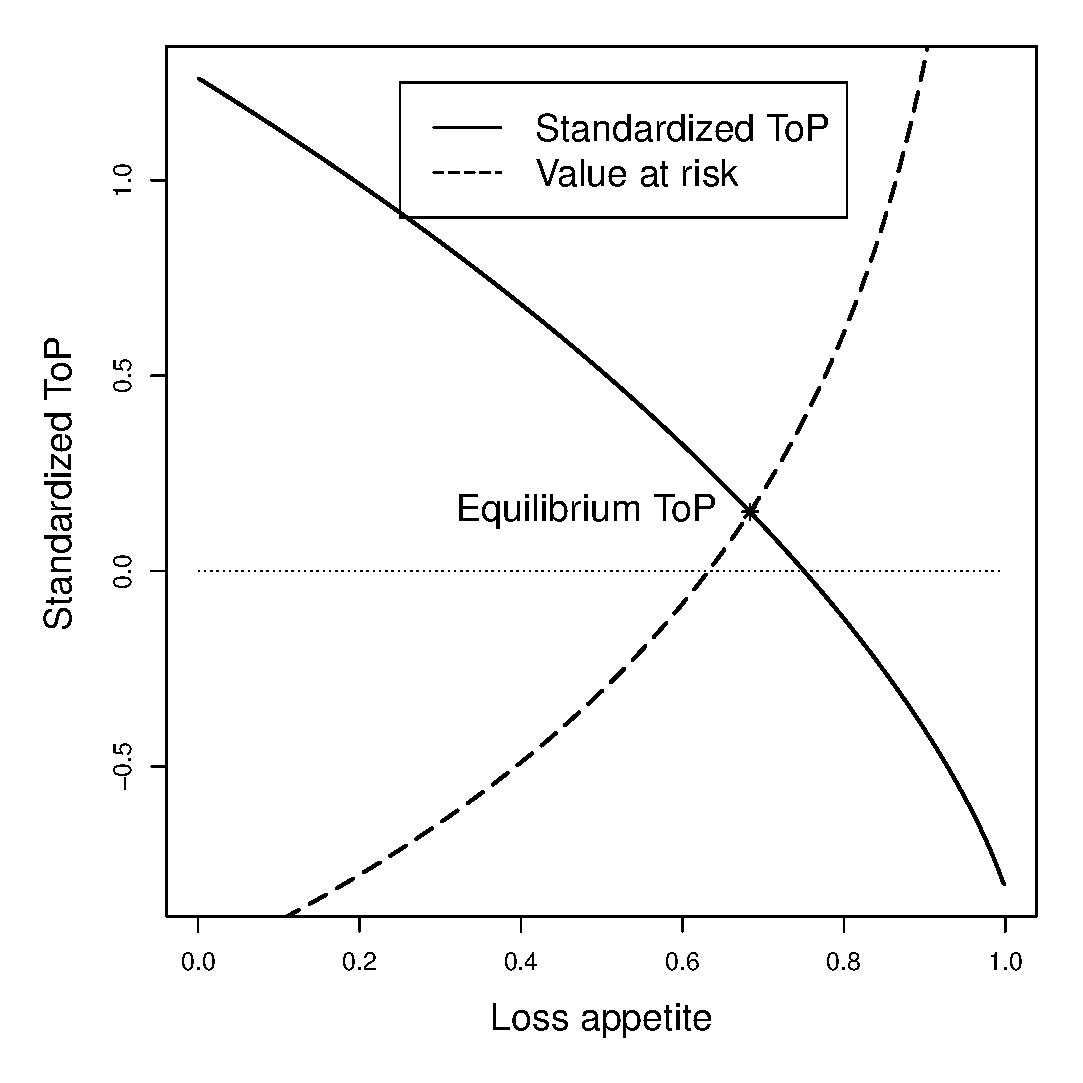
\includegraphics{tradeoffbase.eps}} \\
      \resizebox{60mm}{!}{\includegraphics{varyshape.eps}}
      \resizebox{60mm}{!}{\includegraphics{varyaversion.eps}} \\
    \end{tabular}
    \caption{The top left panel plots penalty weights $\phi_\ell(u)$ against $u$ for various loss appetites $\ell$. The top right panel plots standardised ToP $\top_\ell^*$ and standardised VaR $(V_\ell-\mu_x)/\sigma_x$ against loss appetite $\ell$. The bottom left and right panels plot $\top_\ell^*$ against $\ell$ for varying $\alpha$ and $n$, respectively. Equilibrium ToPs in the bottom panels are indicated by asterisks.}
    \label{illustration}
  \end{center}
\end{figure}








\section{Conclusion}\label{s_conclusion}

The ToP generalises loss aversion reserves, distortion premiums and spectral risks by imposing increasing concern on both smaller and larger loss severities. The formulation is consistent with cumulative prospect theory and the minimisation of pricing error in a competitive market. The loss appetite controls the relative emphasis on small and large severities. Zero loss appetite yields the loss aversion reserve (distortion premium or spectral risk), with sole concern on large severities, while maximum loss appetite yields the dual.

Examples of the ToP using various aversion functions yield two--sided extensions of the well known VaR, conditional--tail--expectation and expected--maximal--loss.



\newpage


\section*{References}

\bibliography{phd}





\end{document}
